\documentclass{article}
\usepackage[utf8]{inputenc}
\usepackage{amsmath}
\usepackage{amssymb}
\usepackage{graphicx}
\usepackage{hyperref}
\usepackage{tikz}
\usepackage{pgfplots}
\usepackage{float}
\usepackage{listings}
\usepackage{color}
\usepackage{bbm}
\usepackage{multirow}
\usepackage{comment}

\newcommand{\wb}{\mathbf{w}}
\newcommand{\xb}{\mathbf{x}}

\title{Reinforcement Learning \\ Exercise 7 - Solution}
\author{Jonathan Schnitzler - st166934 \\
Eric Choquet - st160996}
\date{\today}
\begin{document}
\maketitle

\section{Linear function approximation}

\paragraph*{a)  Tabular linear function approximation}

The method of just writing down all values for each state $V(s)$ can be achieved via the identity as a feature vector, also known as one-hot coding, e.g.
\begin{equation}
    x(s_i) = \begin{pmatrix}
        0 & \hdots & 0 & 1 & 0 & \hdots & 0
    \end{pmatrix}^T.
\end{equation}
This results in the same number as features as states in the state space. The tabular value is now just the weight
\begin{equation}
    V(s) = w_i
\end{equation} and the possible non-linear function $f$ is the identity. The state-action value $Q(s, a)$ could be achieved in a similar way, for $x(s, a) = e_j$ and an according enumeration. The linear function approximation
$$\hat{v}(s,w) = \sum_{i=1}^d w_i f(x_i)$$
is a generalization of the tabular methods.

\paragraph*{b) Update rule for Sarsa}

\begin{enumerate}
\item Tabular case
    $$Q(S_t, A_t) \leftarrow Q(S_t, A_t) + \alpha[R_{t+1} + \gamma Q(S_{t+1}, A_{t+1})- Q(S_t, A_t)]$$
    which is equivalent, shown in task a) to
    $$\mathbf{w}_{t+1} = \mathbf{w}_t + \alpha[R_{t+1} + \gamma \hat{q}(S_{t+1},A_{t+1},\mathbf{w})- \hat{q}(S_t, A_t, \wb_t)]$$
    since there $w_{t,i} = Q(s, a)$
\item Function approximation
$$\mathbf{w}_{t+1} = \mathbf{w}_t + \alpha[R_{t+1} + \gamma \hat{q}(S_{t+1},A_{t+1},\mathbf{w})- \hat{q}(S_t, A_t, \wb_t)]\nabla \hat{q}(S_t, A_t, \wb)$$
\item Linear function approximation
$$\mathbf{w}_{t+1} = \mathbf{w}_t + \alpha[R_{t+1} + \gamma \wb^T \xb(S_{t+1},A_{t+1})- \wb^T \xb(S_t, A_t)] \xb(S_{t}, A_t)$$

% \item Tabular case
% $$\sum_{i=q}^d w_i f(s_{t+1}) = \sum_{i=q}^d w_i f(s_t) +\alpha [R_{t+1} + \gamma (\sum_{i=q}^d w_i f(s_{t+1})) - \sum_{i=q}^d w_i f(s_t)]$$
% \item Function approximation
% $$\sum_{i=q}^d w_i x_i(s_t) = \sum_{i=q}^d w_i x_i(s_t) +\alpha [R_{t+1} + \gamma (\sum_{i=q}^d w_i x_i(s_{t+1})) - \sum_{i=q}^d w_i x_i(s_t)]$$
% \item Linear function approximation\\

\end{enumerate}



\section{Mountain Car}

\begin{comment}
\begin{figure}[H]
\centering
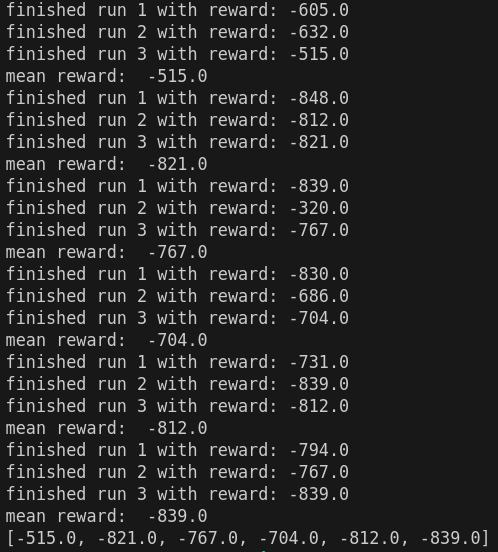
\includegraphics[width=0.5\textwidth]{images/terminal.png}
\caption{Output for Trees with \texttt{maxiter} = [10, 20, 50, 100, 200, 500]}
\label{fig:terminal}
\end{figure}
\end{comment}
TODO:

\end{document}













